\documentclass[12pt]{report}
\usepackage[utf8]{inputenc}
\usepackage[english]{babel}
\usepackage{microtype}
\usepackage{libertine}
\usepackage{amsmath,amsthm}
\usepackage[varg]{newtxmath}\usepackage{setspace,graphicx,epstopdf}
\usepackage{marginnote,datetime,url,enumitem,subfigure,rotating}
\usepackage{todonotes}
\usepackage[open,openlevel=1]{bookmark}
\usepackage[tikz]{bclogo}
\usepackage{enumitem}

\setlength{\parindent}{0ex}
\setlength{\parskip}{1em}%Espacement des par

\setlist[itemize]{topsep= -5pt, itemsep=-1.5pt}
\setlist[enumerate]{topsep= -5pt, itemsep=-1.5pt}

\def\D{\mathrm{d}}

\newtheorem{theorem}{Theorem}[chapter]
\newtheorem{definition}{Definition}[chapter]
\newtheorem{proposition}{Proposition}[chapter]
\newtheorem{axiom}{Axiom}[chapter]

\newcommand{\smalltodo}[2][] {\todo[caption={#2}, size=\scriptsize,%
fancyline, #1]{\begin{spacing}{.5}#2\end{spacing}}}
\newcommand{\rhs}[2][]{\smalltodo[color=green!30,#1]{{\bf PS:} #2}}

\renewcommand\bcStyleTitre[1]{\textbf{#1}}

\begin{document}

\date{}
\title{ECON7740 - Microeconomic Th. I\\ Lecture Notes}
\author{Paul Anthony Sarkis\\ Boston College} 
 
\maketitle

\tableofcontents

\chapter{Choice, Preferences and Utility}

\section{From Choice to Preference}

In this course, we will study the basics of individual choice: how people choose when presented different alternatives. Let $X$ denote the set of possible alternatives $x$.

Typically, we have seen that people make choices according to a concept of utility, a function to be maximized. Specifically, $u(\cdot):X\to \mathbb{R}$ so that $x$ is chosen over $y$ if $u(x)>u(y)$.

These choices over a set of different possibilities are observable by the economist, we call them primitive data. The real challenge is however to use the data to infer meaningful information about the true preferences of individuals. We talk about revealing an individual's preferences. How can we do it?

\begin{definition}
A choice structure $(\mathcal{B},C)$ consists of:\begin{itemize}
\item A set $\mathcal{B}$ of choice sets $B\subseteq X$,
\item and a mapping $C:\mathcal{B}\to X$, called a choice rule, that maps each $B\in\mathcal{B}$ to a non-empty set $C(B)\in X$.
\end{itemize}
\end{definition}
The resulting set $C(B)$ is the set of chosen alternatives when $B$ is proposed.

\begin{definition}
A preference relation, denoted $\succeq$ is a binary relation defined over the set $X$. In particular, for any $x,y\in X$, $x\succeq y$ means that $x$ is weakly preferred to $y$.

We define the relation of strict preference, $\succ$ as: $x\succ y \Leftrightarrow x\succeq y$ but $y \not\succeq x$ ; and the relation of indifference $\sim$ as: $x\sim y \Leftrightarrow x \succeq y$ and $y \succeq x$. 
\end{definition}

In order to advance in our analysis, we will need to use and explain some basic axioms (assumptions) on this preference relation.

\begin{axiom}[Completeness]
A preference relation $\succeq$ is said to be complete over $X$ if for all $x,y\in X$, we have either $x\succeq y$ or $y \succeq x$.
\end{axiom}

\begin{axiom}[Transitivity]
A preference relation $\succeq$ is said to be transitive over $X$ if for all $x,y,z\in X$, $x\succeq y$ and $y \succeq z$ implies $x\succeq z$.
\end{axiom}

\begin{definition}[Rationality]
When a preference relation $\succeq$ satisfies both axioms of completeness and transitivity, we say that the preference relation is rational.
\end{definition}

\begin{proposition}
If a preference relation $\succeq$ is rational over $X$, then $\succ$ and $\sim$ are transitive over $X$.
\end{proposition}

\begin{proof}
Assume that $x\succ y$ and $y\succ z$ but $x\not\succ z$. Using the completeness of $\succeq$, this implies that $z\succeq x$. Moreover, because $x\succeq y$, by transitivity of $\succeq$, we must have that $z\succeq y$, which is a contradiction.

Now assume that $x\sim y$ and $y\sim z$ but $x\not\sim z$. This implies that either $x\succeq z$ and $z \not\succeq x$, or $z\succeq x$ and $x\not\succeq z$. In the first case, $y\succeq z$ but $z \not\succeq x$, therefore $y\not\succeq x$, a contradiction. In the second case, $y \succeq x$ but $x\not\succeq z$, implying that $y\not\succeq x$, another contradiction.
\end{proof}

\begin{definition}
Let $B$ be any subset of $X$. An optimal choice set $C^*(B, \succeq)$ is the set consisting of all choices weakly preferred to any other option. $$C^*(B, \succeq) = \{x\in B: x\succeq y, \forall y\in B\}$$ We say that $\succeq$ rationalizes $(\mathcal{B},C)$ if $C(B) = C^*(B,\succeq)$ for all $B\in\mathcal{B}$. In words, $\succeq$ rationalizes the choice data if the set of optimal choices is equal to the set of observed choices.
\end{definition}

\begin{definition}
Given the choice data $(\mathcal{B}, C)$, the revealed preference relation $\succeq^*$ is defined by: $$ x\succeq^*y \Leftrightarrow \exists B\in\mathcal{B}\text{ with } x,y\in B\text{ and } x\in C(B) $$ If $x\in C(B)$ for all $B\in\mathcal{B}$, then $x$ is weakly revealed preferred to $y$.\\ \\
If $\exists B\in\mathcal{B}$ for which $x,y\in B$, $x\in C(B)$ and $y\not\in C(B)$, then $x$ is strictly revealed preferred to $y$.
\end{definition}

\begin{axiom}[Weak Axiom of Revealed Prefernces]
Choice data $(\mathcal{B}, C)$ satisfies WARP if for any $x$ weakly revealed preferred to $y$, $y$ cannot be strictly revealed preferred to $x$.
\end{axiom}

\begin{theorem}
If choice data $(\mathcal{B}, C)$ satisfies WARP and $\mathcal{B}$ includes at least all subsets $B$ of $X$ of at least three elements, then $\succeq^*$ is rational and is the only preference relation that rationalizes $(\mathcal{B}, C)$.\\If  $(\mathcal{B}, C)$ violates WARP, then there can be rational preference relation that rationalizes the choice data.
\end{theorem}

\section{Preference and Utility}

Now that we know how to infer preference from choice data, we can use preference to try and map them on the real line, thanks to the utility function.

\begin{definition}
A utility function, $u:X\to\mathbb{R}$, represents a preference relation $\succeq$ defined on $X$ if, for all $x,y\in X$,$$x\succeq y \Leftrightarrow u(x)\geq u(y)$$
\end{definition}

The only information revealed by a preference relation is an order of the elements of $X$; we talk about an ordinal property. Utility, using the real line, call upon a cardinal property (where distances between elements have a signification). We cannot use the latter property to describe an individual's preference. You should see utility numbers as describing an order only.

\begin{proposition}
If a utility function $u(\cdot)$ represents the preference relation $\succeq$ on $X$. Then, any monotonic transformation $g(\cdot)$ of $u(\cdot)$ will also represent $\succeq$.
\end{proposition}

\begin{proof}
From the properties of a monotonic transformation, $g(u(x))\geq g(u(y))$ if and only if $u(x)\geq u(y)$, therefore it must represent $\succeq$. 
\end{proof}

\begin{theorem}
Only rational preference relations can be represented as utility functions. Conversely, if $X$ is finite, then any preference relation can be represented by a utility function.
\end{theorem}

\begin{axiom}[Continuity]
For $X\subseteq\mathbb{R}^n$, a preference relation $\succeq$ is said to be continuous on $X$ if, for all $\{x^m\}\to x$ and $\{y^m\}\to y$ in $X$ such that $x^m\succeq y^m$ for all $m$, we have $x\succeq y$.
\end{axiom}

\begin{theorem}
For $X\subseteq\mathbb{R}^n$, any continuous and rational preference relation can be represented by a utility function.
\end{theorem}

\begin{bclogo}[couleur=blue!10, arrondi=0.1, logo=,ombre=false]{ Lexicographic Preferences} 
\begin{small}
Let $X$ be the set $[0,1]\times [0,1]$. The preference relation $\succeq$ is defined by $(x_1, x_2)\succeq (y_1, y_2)$ if either: $x_1>y_1$ or $x_1 = y_1$ and $x_2 > y_2$. In words, the element with the highest first component is preferred. If there is a tie, then the element with the highest second component is preferred.

Lexicographic preferences are not representable by any utility function. \begin{proof}
Not continuous, show counter example
\end{proof}
\end{small}
\end{bclogo}

The three assumptions we have seen about preference relations are the least we can use in order to characterize a utility function to maximize. Doing useful analysis entails having to make that kind of assumptions. Nevertheless, we should be very careful about adding assumptions to a model. You should always try to understand what those assumptions mean in terms of behavior, use the clearest, simplest and least restrictive assumptions in your models.

In order to push a bit further on utility, preference and choices, we will add some assumptions, explaining every implications along the way.

\begin{axiom}[Monotonicity]
A preference relation $\succeq$ is said to be monotone if for all $x,y\in X$ such that $x\geq y$, we have $x\succeq y$.\\ \\ It is said to be strictly monotone if $x>y$ implies $x\succ y$.
\end{axiom}

\begin{proposition}
Suppose a preference relation $\succeq$ is represented by the utility function $u(\cdot)$. Then, $$u(\cdot)\textit{ is non-decreasing }\Leftrightarrow \textit{ }\succeq \textit{ is monotone} $$ and $$u(\cdot)\textit{ is strictly increasing }\Leftrightarrow \textit{ }\succeq \textit{ is strictly monotone.} $$
\end{proposition}

\begin{proof}

\end{proof}

\begin{definition}[Open balls]
Let $x$ be any option in $X$. We define an open-ball neighborhood around $x$ such that $$B_{\varepsilon}(x) = \{ y\in X: \lVert x - y \rVert < \varepsilon \} $$ It represents the set of all elements in $X$ that are at a smaller distance than $\varepsilon$ from $x$.
\end{definition}

\begin{axiom}[Local-Nonsatiation]
A preference relation $\succeq$ is said to be locally non-satiated if, for any $x\in X$ and $\varepsilon >0$, there exists $y\in B_{\varepsilon}(x)$ such that $y\succ x$.
\end{axiom}

\begin{proposition}
Suppose a preference relation $\succeq$ is represented by the utility function $u(\cdot)$. Then, $$ u(\cdot)\textit{ has no local maximum }\Leftrightarrow \textit{ }\succeq \textit{ is LNS.} $$
\end{proposition}

\begin{proof}

\end{proof}

\begin{axiom}[Convexity]
A preference relation $\succeq$ is said to be convex if $x\succeq y$ and $x'\succeq y$ imply that for any $\alpha\in (0,1)$, $$\alpha x + (1 - \alpha)x' \succeq y $$ It is said to be strictly convex if when $x\neq x'$, we have: $$\alpha x + (1 - \alpha)x' \succ y $$ 
\end{axiom}

\begin{definition}[Contour sets]
For any $x\in X$, the upper contour set, denoted $U(x)$ is the set of all options $y\in X$ such that $y\succeq x$. The lower contour set, denoted $L(x)$ is the set of all $y\in X$ such that $x\succeq y$. \begin{align*}
U(x) & = \{y\in X : y\succeq x\} \\
L(x) & = \{y\in X : x\succeq y\}
\end{align*}
\end{definition}

\begin{proposition}
A preference relation $\succeq$ is convex if and only if, for all $x\in X$, $U(x)$ is a convex set.
\end{proposition}

\begin{proof}

\end{proof}

\begin{theorem}
Let $\succeq$ be any convex preference relation. Then, for any convex choice set $B$, the set $C^*(B,\succeq)$ is also convex.

If $\succeq$ is strictly convex, then the set $C^*(B,\succeq)$ is either single-valued or empty.
\end{theorem}

\begin{proof}

\end{proof}

\begin{definition}[Quasi-concavity]
A function $u:X\to\mathbb{R}$ is quasi-concave if, for every $x,y\in X$ such that $u(x)\geq u(y)$ and any $\alpha\in(0,1)$ we have that, $$u(\alpha x + (1-\alpha) y)\geq u(y)$$It is strictly quasi-concave if for $x\neq y$, $$u(\alpha x + (1-\alpha) y)> u(y)$$
\end{definition}

\begin{proposition}
Suppose a preference relation $\succeq$ is represented by the utility function $u(\cdot)$. Then, $$u(\cdot)\textit{ is quasi-concave }\Leftrightarrow \textit{ }\succeq \textit{ is convex} $$ and $$u(\cdot)\textit{ is strictly quasi-concave }\Leftrightarrow \textit{ }\succeq \textit{ is strictly convex.} $$
\end{proposition}

\begin{proof}

\end{proof}

\begin{definition}[Weak Separability]
Let $J_1,...J_m$ be a list of $m$ mutually exclusive subsets of $X$. Define $J_k^C$ as the complement of the set $J_k$. Finally, we denote $x_{J_k}$ the elements of $x$ included in $J_k$.

A preference relation $\succeq$ is said to be weakly separable in $J_1, ... J_m$ if, for every $k$ and every $x_{J_k}, x'_{J_k}$, $$(x_{J_k},x_{J_k^C})\succeq (x'_{J_k},x_{J_k^C}) \Leftrightarrow (x_{J_k},x'_{J_k^C})\succeq (x'_{J_k},x'_{J_k^C}) $$ In words, this implies that a preference relation between two options in the same subset does not depend on options in other subsets.
\end{definition}

\chapter{Consumer Theory}

\section{Utility Maximization Problem (UMP)}

Let's review this problem by setting up the context:\begin{itemize}
\item The consumer chooses a consumption vector $x = (x_1, ..., x_n)\in X$ where $x_k$ denotes the level of consumption of good $k$\begin{itemize}
\item[$\Rightarrow$] $x\in\mathbb{R}_{+}^n$, which means it can be any positive real value, implying goods can be indefinitely divisible.
\end{itemize}
\item He tries to achieve the maximum utility $u(x)$.
\item For each unit of good $k$ he has to pay a price $p_k$.\begin{itemize}
\item[$\Rightarrow$] $p_k$ is the same for any quantity $x_k$ consumed: we say that prices are linear.
\item[$\Rightarrow$] $p_k$ is assumed to be positive for all $k$.
\end{itemize}
\item His total available income is $w$.
\end{itemize} 
We can set up the problem in mathematical terms as,$$\max_{x\in X} u(x) \text{ s.t. } px \leq w $$

\begin{definition}[Budget set]
We define the budget set of a consumer as $$B(p,w) = \{x\in \mathbb{R}_{+}^n : px\leq w\} $$This is the set containing all affordable bundles of goods. The set can also be defined by the boundary hyperplane, called the budget line: $$px = w$$
\end{definition}

\begin{definition}[Marshallian demand correspondence]
The solution to the utility maximization problem is a correpondence $x:\mathbb{R}_{+}^n \times \mathbb{R} \rightrightarrows \mathbb{R}_{+}^n $ such that: \begin{align*}
x(p, w) & = \operatorname{arg}\max_{x\in B(p,w)} u(x) \\
& = \{z\in B(p,w):u(z) = \max_{x\in B(p,w)} u(x)\}
\end{align*}
\end{definition}

The two previous definitions imply a set of interesting properties that can be interpreted nicely in the UMP context.

\begin{theorem}[Homogeneity of the budget set]
Any budget set is homogeneous of degree $0$: that is, for all $\lambda >0$, $B(\lambda p, \lambda w) = B(p, w)$. In words, if income and prices are scaled by the same factor, the set of affordable goods remains exactly the same.
\end{theorem}

\begin{proof}
\begin{align*}
B(\lambda p, \lambda w) & = \{x\in \mathbb{R}_{+}^n : (\lambda p)x\leq \lambda w\} \\ & = \{x\in \mathbb{R}_{+}^n : px\leq w\} \\ & = B(p, w)
\end{align*}
\end{proof}

\begin{theorem}[Compactness of the budget set]
If $p\gg 0$, then $B(p, w)$ is a compact ($=$ closed and bounded) set.
\end{theorem}

\begin{proof}
We already know, by definition, that $B(p, w)$ is closed. Now, if $p\gg 0$, we also have that the budget set is bounded below by $0$, and above by $w$.
\end{proof}

\begin{theorem}[Existence of the demand correspondence]
If $u(\cdot)$ is a continuous function on $X$ and $p\gg 0$, then the Marshallian demand correspondence $x(p,w)$ is non-empty: the UMP admits at least one solution.
\end{theorem}

\begin{proof}
This follows directly from the Extreme Value theorem stating that any continuous function on a compact set must admit at least one maximum and one minimum point.
\end{proof}

\begin{theorem}[Properties of Marshallian Demand]
If the UMP admits a solution in the form of a Marshallian demande correspondence, then the correspondence possess these following properties:\begin{itemize}
\item \textbf{Homogeneity of degree $0$:} for all $\lambda >0$, $x(\lambda p, \lambda w) = x(p,w)$.
\item \textbf{Walras' Law:} if preferences are LNS, then for any $(p,w)$ and any point in $z\in x(p,w)$, we have that $pz = w$. This result implies that the the demand correspondence must lie on the budget line.
\item \textbf{Convexity:} if the demand correspondence is not single-valued, then it is convex, meaning that if $x, x'\in x(p,w)$, then for all $\sigma\in(0,1)$, we have that $\sigma x + (1-\sigma) x'\in x(p,w)$ as well.
\item \textbf{Differentiability:} if the demand correspondence is single-valued and differentiable, then we get a set of three interesting properties:\begin{enumerate}
\item A proportional change in all prices and income will not affect demand: $$\sum_{j=1}^{n} p_j\frac{\partial}{\partial p_j} x_i(p,w) + w\frac{\partial}{\partial w}x_i(p,w) = 0 $$
\item A change in the price of one good does not affect total expenditure: $$\sum_{j=1}^{n} p_j\frac{\partial}{\partial p_j} x_i(p,w) + x_i(p,w) = 0 $$
\item A change in income leads to an identical change in total expenditure: $$\sum_{i=1}^{n} p_i\frac{\partial}{\partial w} x_i(p,w) = 1 $$
\end{enumerate}
\end{itemize}
\end{theorem}
\begin{proof}
(Homogeneity of degree 0): This is trivial since the budget set is homogeneous of degree 0 as well. If $x^*\in B(p,w)$, then $x^*\in B(\lambda p,\lambda w)$.

(Walras' Law): Let $x\in x(p,w)$. If $px<w$, then there exists an $\varepsilon>0$ such that $B_\varepsilon(x)\subseteq B(p,w)$. By LNS, for all $\varepsilon>0$, $\exists y\in B_\varepsilon(x)$ such that $y\succ x$, implying that $y\in B(p,w)$: a contradiction of the optimality of $x$.

(Convexity): Again, trivially, by convexity of the budget set, it must be that $x(p,w)$ is convex.

(Differentiabilty): i. By Euler's theorem, since demand is a homogeneous function of degree zero, it must be that the sum of all derivatives times their own variable is equal to the degree of homogeneity.

ii.

iii. Trivially, by differentiating the equation of Walras' law: $$\sum_{i=1}^{n}\frac{\partial}{\partial w} p_ix_i(p,w) = 1$$
\end{proof}

\begin{definition}[Indirect Utility Function]
The indirect utility function $v:\mathbb{R}^{n+1}\to\mathbb{R}$ is defined as the value function of the UMP: $$v(p,w) = \max_{x\in B(p,w)} u(x) $$
\end{definition}

\begin{theorem}[Properties of the indirect utility function]
The indirect utility function satisfies the following properties:\begin{itemize}
\item \textbf{Homogeneity of degree 0:} for all $\lambda > 0$, $v(\lambda p, \lambda w) = v(p,w)$.
\item \textbf{Continuity:} if $u$ is a continuous function, then $v$ is continuous on $(p,w)$.
\item \textbf{Monotonicity:} $v(p,w)$ is a non-increasing function in $p$ and a non-decreasing function in $w$. If preferences are LNS, then $v(p,w)$ is strictly increasing in $w$.
\item \textbf{Quasi-convexity:} for all $\bar v\in\mathbb{R}$, the lower-level set of $v(p,w)\leq \bar v$ is convex.
\end{itemize}
\end{theorem}

Before going further into the properties of the indirect utility function, recall some properties of value functions, coming from the Kuhn-Tucker and Envelope theorems. In our context, suppose $u$ is LNS and continuously differentiable and $x$ is single-valued for all $(p,w)$. Then, $v(p,w)$ is continuously differentiable at $(p,w)$. In particular, at the optimal $x^*\in x(p,w)$, we have: $$\frac{\partial}{\partial w}v(p,w) = \lambda = \frac{1}{p_i}\frac{\partial}{\partial x_i}u(x^*) $$ $$\frac{\partial}{\partial p_i}v(p,w) = -\lambda x_i^* = \frac{x_i^*}{p_j}\frac{\partial}{\partial x_j}u(x^*) $$ Those two results will help us in proving Roy's identity, but they also tell us something really nice about how consumers react to shocks in income or prices:\begin{itemize}
\item From the first equation, the effect of a variation of 1\$ in income is exactly equal to the variation in the amount of a good times its marginal utility.
\item The effect of a variation of 1\$ in the price of a good will have the same effect as a change of income.
\end{itemize}

\begin{theorem}[Roy's identity]
If $x_i(p,w)>0$, then $$x_i(p,w) = -\frac{\frac{\partial}{\partial p_i}v(p,w)}{\frac{\partial}{\partial w}v(p,w)} $$
\end{theorem}
\begin{proof}
Trivially, from the results derived above: $$-\frac{\frac{\partial}{\partial p_i}v(p,w)}{\frac{\partial}{\partial w}v(p,w)} = - \frac{-\lambda x_i^*}{\lambda} = x_i(p,w) $$
\end{proof}

\section{Expenditure Minimization Problem}

In the previous section we have seen a consumer that tries to maximize his utility while under a budget constraint. Another problem that he might face would be the opposite: trying to minimize his expenditures subject to a minimum utility constraint. This is the Expenditure minimization problem (EMP). It is set up formally as: $$\min_{x\in\mathbb{R}_{+}^n} p\cdot x \text{ s.t } u(x)\geq \bar u $$

\begin{definition}[Hicksian demand correspondence]
The solution to the EMP is a correpondence $h:\mathbb{R}_{+}^n \times \mathbb{R} \rightrightarrows \mathbb{R}_{+}^n $ such that: \begin{align*}
h(p, u) & = \operatorname{arg}\min_{x\in\mathbb{R}_{+}^n:u(x)\geq\bar u} p\cdot x \\
& = \{z : u(z)\geq\bar u\text{ and } p\cdot z = \min_{x} p\cdot x\}
\end{align*}
\end{definition}

\begin{theorem}[Properties of Hicksian Demand]
If the EMP admits a solution in the form of a Hicksian demand correspondence, then the correspondence possess these following properties:\begin{itemize}
\item \textbf{Homogeneity of degree $0$:} for all $\lambda >0$, $h(\lambda p, u) = h(p,u)$.
\item \textbf{No excess utility:} if $u(\cdot)$ is continuous and $p>0$, then $u(x) = \bar u$ for all $x\in h(p,u)$.
\item \textbf{Convexity:} if preferences are convex, then the Hicksian demand correspondence is convex, meaning that if $x, x'\in h(p,u)$, then for all $\sigma\in(0,1)$, we have that $\sigma x + (1-\sigma) x'\in h(p,u)$ as well. If preferences are strictly convex then $h(p,u)$ is single-valued.
\end{itemize}
\end{theorem}

\begin{definition}[Expenditure function]
The expenditure function, $e(p,u)$, is the value function of the EMP. Formally, $$e(p,u) = \min_{x\in\mathbb{R}_{+}^n:u(x)\geq\bar u} p\cdot x$$
\end{definition}

\begin{theorem}[Properties of the expenditure function]
The expenditure function satisfies the following properties:\begin{itemize}
\item \textbf{Homogeneity of degree 1 in $p$:} for all $\lambda > 0$, $e(\lambda p, u) = \lambda e(p,u)$.
\item \textbf{Continuity:} if $u$ is a continuous function, then $e$ is continuous in $p$ and $u$.
\item \textbf{Monotonicity:} $e(p,u)$ is a non-decreasing function in $p$ and a non-decreasing function in $u$. If $u(\cdot)$ is continuous and $p>0$, then $e(p,w)$ is strictly increasing in $u$.
\item \textbf{Concavity in $p$:} $e(p,u)$ is concave in $p$.
\end{itemize}
\end{theorem}

These concepts are connected to the UMP as we'll see later, but they can teach us important elements of the dynamics of our model. In fact, the Hicksian demand is useful for studying effects of price changes on "real" demand, whereas the Marshallian demand is affected by both income and substitution effects. The expenditure function will also be important for welfare analysis.

Again, before going further into the properties of the expenditure function, we'll analyze the Kuhn-Tucker and Envelope theorems in this context. Suppose $u$ is LNS and continuously differentiable and $h(p,u)$ is single-valued for all $(p,u)$. Then, $e(p,u)$ is continuously differentiable at $(p,u)$. In particular, at the optimal $h^*\in h(p,u)$, we have: $$e(p,u) = p\cdot h^* + \lambda^*[u(h^*) -\bar u] $$ $$\Rightarrow \frac{\partial}{\partial p_i}e(p,u) = h_i^* $$ This result is sometimes referred to as Shephard's lemma. It provides an interesting insight on consumer behavior: if the price of a good increases by $1$ dollar, then the optimal bundle will cost $h_i(p,u)$ more dollars.

\section{Comparative Statics}

Comparative statics are statements about how the solution of a problem changes with regards to variations or shocks in the parameters. In the UMP, our solutions are $x(p,w)$ and $v(p,w)$ so we might be interested in how they change after shocking $p$ or $w$. In the EMP, our solutions are $h(p,u)$ and $e(p,u)$, so we will look for changes following shocks to $p$ and $u$. The comparative statics of the EMP are much simpler than those of the UMP, hence we'll start with those and see if they can help us understand more the UMP problem.

\subsection{Comparative statics of the EMP}

\begin{theorem}[Law of demand]
For any $p,p' \geq 0$, $x\in h(p,u)$ and $x'\in h(p',u)$, we have: $$(p' - p)(x' - x)\leq 0$$ which means that $h(p,u)$ is always decreasing in prices.
\end{theorem}

\begin{definition}[Slutsky Matrix]
If the Hicksian demand is single-valued and differentiable, the Slutsky matrix is the matrix of price-derivatives: \begin{equation*}
D_p h(p,u) = \begin{bmatrix}
\frac{\partial}{\partial p_1}h_1(p,u) & \hdots &  \frac{\partial}{\partial p_1}h_n(p,u) \\
\vdots & \ddots & \vdots \\
\frac{\partial}{\partial p_n}h_1(p,u) & \hdots &  \frac{\partial}{\partial p_n}h_n(p,u)
\end{bmatrix}
\end{equation*}
\end{definition}

\begin{theorem}[Properties of the Slutsky matrix]
If $h(p,u)$ is single-valued and continuously differentiable in $p$ at the point $(p,u)$, then $D_ph(p,u)$ is symmetric and negative semi-definite.
\end{theorem}
\begin{proof}
From Shephard's lemma, we have that $h_i = \frac{\partial}{\partial p_i}e(p,u)$, therefore, $\frac{\partial}{\partial p_j}h_i = \frac{\partial^2}{\partial p_i\partial p_j}e(p,u)$. Then from Young's theorem we have symmetry of $D_ph(p,u)$. Now, if you choose any vector $z = (z_1, ..., z_i, ... z_n) = (0, ..., 1, ..., 0)$ you would have that $z'D_ph(p,u)z = \frac{\partial}{\partial p_i}h_i(p,u) \leq 0$ hence the negative semi-definite matrix. 
\end{proof}

This theorem might seem useless but really it gives an interesting insight: changing the price of $j$ has the same effect on $h_i$ than the same variation of $i$ on $h_j$. This is not true with Marshallian demand because of income effects that might come into play.

\subsection{Comparative statics of the UMP}

Now that we know how Hicksian demand behaves, we'll try and relate to the Marshallian demand.

\begin{theorem}[Duality of the UMP and EMP]
Suppose $u(\cdot)$ is continuous and locally non-satiated. Then,\begin{itemize}
\item For all $p>0$ and $w\geq 0$, $x(p,w) = h(p, v(p,w))$ and $e(p,v(p,w)) = w$.
\item For all $p>0$ and $u\geq 0$, $h(p,u) = x(p, e(p,u))$ and $v(p,e(p,u)) = u$.
\end{itemize}
\end{theorem}

\begin{theorem}[Slutsky equation]
Suppose $u(\cdot)$ is continuous and locally non-satiated. Let $p>0$ and $w = e(p,u)$. If $x(p,w)$ and $h(p,u)$ are single-valued and differentiable, then: $$\underbrace{\frac{\partial x_i(p,w)}{\partial p_j}}_{\text{Total effect}} = \underbrace{\frac{\partial h_i(p,u)}{\partial p_j}}_{\text{Substitution effect}}  \underbrace{- x_j(p,w)\cdot\frac{\partial x_i(p,w)}{\partial w}}_{\text{Income effect}} $$ $$ \text{Total effect} = \text{Substitution effect} + \text{Income effect} $$
\end{theorem}

The intuition from this theorem is quite neat:\begin{itemize}
\item \textbf{Substitution effect:} $\frac{\partial h_i(p,u)}{\partial p_j}$ represents the movement along the indifference curve. It is the response to a change in prices, keeping $u$ fixed.
\item \textbf{Income effect:} $- x_j(p,w)\cdot\frac{\partial x_i(p,w)}{\partial w}$ represents the movement from one indifference curve to another. It is the response to a change in income, keeping $p$ fixed.
\end{itemize}

\begin{definition}[Normal and inferior goods]
A good $i$ is said to be a normal good if $x_i(p,w)$ is increasing in $w$. It is inferior if $x_i(p,w)$ is decreasing in $w$.
\end{definition}

\begin{definition}[Regular and Giffen goods]
A good $i$ is said to be a regular good if $x_i(p,w)$ is decreasing in $p$. It is a Giffen good if $x_i(p,w)$ is increasing in $p$.
\end{definition}

\begin{definition}[Substitutes and complements]
A good $i$ is said to be a substitute for good $j$ if $h_i(p,u)$ is increasing in $p_j$. It is a complement of good $j$ if $h_i(p,u)$ is decreasing in $p_j$.
\end{definition}

\section{Welfare effects of price changes}

In this part of the chapter, we'll turn our interest to changes of consumer welfare following changes of parameters of the model, and in particular changes of $p$. The question we want to answer is straightforward, what happens to utility when prices change from $p$ to $p'$.

The answer is obvious as well, in a perfect world we would measure the indirect utility function at the two price points and compute the difference. However, how can we measure utility? It's impossible because of its ordinality (no cardinality): differences in utility only indicate preferences, not the magnitude of preferences. This is why we need to shift our focus to a measurable variable, money!

This class of measures are called money-metric indirect utility functions. They can be constructed through the expenditure function such as: $e(p, v(p,w))$. In fact, we know that the expenditure function is increasing in $u$ so it will represent preferences correctly (thus it is actually also an indirect utility function).

The measure we'll use is based on the following equation: $$e(\bar p, v(p', w)) - e(\bar p, v(p, w)) $$ This measure is independent of the choice of $v$ since it represents only an expenditure on a set that is satisfied by all correct indirect utility functions. Now we only need to specify $\bar p$. This starting point allows for two methods: equivalent variation (EV) and compensating variation (CV).

\subsection{Equivalent variation}

EV measures the required expenditure change at the original price $\bar p = p$. Hence, it is a measure of the amount of money that you would need to give a consumer at $p$ in order to make him indifferent of changing to $p'$. This amount is equivalent of going through the price change. Formally, \begin{align*} 
EV = e(p, v(p',w)) - e(p, v(p,w)) & = e(p, v(p',w)) - w \\
& = e(p, v(p',w)) - e(p', v(p',w)) \\
& = \int_{p'}^{p} h(p, v(p',w))\D p
\end{align*}

\subsection{Compensating variation}

CV measures the required expenditure change at the changed price $\bar{p} = p'$. Hence, it is a measure of the amount of money that would you would need to give a consumer at $p'$ in order to make him indifferent of having changed to $p'$. This amount compensates going through the price change. Formally, \begin{align*} 
CV = e(p', v(p',w)) - e(p', v(p,w)) & = w - e(p', v(p,w)) \\
& = e(p, v(p,w)) - e(p', v(p,w)) \\
& = \int_{p'}^{p} h(p, v(p,w))\D p
\end{align*}

\chapter{Theory of the firm}

\section{Production}

Again, we'll start by setting up the context in order to have a clearer view of how the defined tools are going to help us solve the firm's problem. Production is the process of transforming inputs into outputs, this process is heavily reliant on the concept of technological feasability. Indeed, the technology will determine and restrict what is possible to create using a set of input. We set $Y\subset\mathbb{R}^m$ as being the production possibility set: the set of all feasible combinations of inputs and outputs. The vector $y = (y_1, ..., y_m)\in Y$ is the production plan of the firm. We use $y_i < 0$ to denote an input, while $y_i > 0$ will define our output. When there are only one output for many inputs, we'll divide them in two $x = (x_1, ..., x_n)$ for inputs and $y$ for output.

\begin{definition}[Production function]
The production function $f:\mathbb{R}_+^n\to\mathbb{R}$ is continuous, strictly increasing and strictly quasiconcave on $\mathbb{R}_+^n$, and $f(0) = 0$.
\end{definition}

\begin{definition}[Marginal product]
If the production function is differentiable, its derivative with respect to input $i$ is called the marginal product of input $i$, denoted $MP_i$: $$MP_i(x) = \frac{\partial f(x)}{\partial x_i} $$
\end{definition}

\begin{definition}[Isoquant]
For any fixed level of output $y$, the set of input vectors $x$ that produce $y$ is called the $y$-level isoquant of $f$. We denote it by $Q(y)$, $$Q(y) = \{x\geq 0 : f(x) = y\} $$
\end{definition}

The isoquant is really helpful for identifying the set of inputs leading to the same level of output, however, it does give any indication on the amount of input $i$ we might want to substitute for $j$ to keep the same level of output. This measure can be given by two variables described below:

\begin{definition}[Marginal rate of technical substitution]
The MRTS is the analogue of the MRS for the consumer problem. It is a measure of the rate at which one input $i$ can be substituted with another input $j$ while keeping the ouput level constant. We denote it $MRTS_{ij}(x)$, $$MRTS_{ij}(x) = \frac{\partial f(x)/\partial x_i}{\partial f(x)/\partial x_j} $$ If the production is separable, then the MRTS of two inputs does not depend on the level of any other inputs.
\end{definition}

\begin{definition}[Elasticity of substitution]
For a production function $f(x)$, the elasticity of substitution of input $j$ for input $i$ at a point $x^0$ is defined as: $$\sigma_{ij}(x^0) = \left(\frac{\D\ln(MRTS_{ij}(x(r)))}{\D\ln(r)}\right)^{-1} $$ where $x(r)$ is the vector of inputs such that $x_j/x_i = r$, $x_k = x_k^0$ for all $k\neq i,j$ and $f(x(r)) = f(x^0)$.
\end{definition}


Finally, the last topic we'll study around production functions are returns to scale. This topic is the study of how much the output varies as the amounts of inputs vary. We'll have to define a few concepts first before delving into returns to scale.

\begin{definition}[Average product]
The average product of an input $i$ is defined by the average amount of output produced for each unit of the input $i$, we denote it $AP_i(x)$, $$AP_i(x) = \frac{f(x)}{x_i} $$.
\end{definition}

\begin{definition}[Output elasticity of input $i$]
The output elasticity of input $i$ is a measure of the percentage variation of output to a a 1\% change in the input $i$, we denote it $\mu_i(x)$, $$\mu_i(x) = \frac{\partial f(x)}{\partial x_i}\frac{x_i}{f(x)} = \frac{MP_i(x)}{AP_i(x)} $$
\end{definition}

Now we can turn to returns to scale, which we'll identify two types of.

\begin{definition}[Global returns to scale]
A production function $f(x)$ has the property of:\begin{itemize}
\item Constant returns to scale (CRS) if $f(\lambda x) = \lambda f(x)$ for all $\lambda > 0$ and all $x$.
\item Increasing returns to scale (IRS) if $f(\lambda x) > \lambda f(x)$ for all $\lambda > 0$ and all $x$.
\item Decreasing returns to scale (DRS) if $f(\lambda x) < \lambda f(x)$ for all $\lambda > 0$ and all $x$.
\end{itemize}
\end{definition}

%ONE DEF MISSING

\section{Cost}

\begin{definition}[Cost function]
The cost function $\mathcal{C}:\mathbb{R}^{n+1}\to \mathbb{R}$, defined for all input prices $w$ and all output levels $y$ is the minimum-value function: $$\mathcal{C}(w,y)\equiv \min_{x} w\cdot x\text{ s.t. } f(x)\geq y $$ 
\end{definition}

\begin{definition}[Conditional input demand]
Let $x^*(w,y)$ be the solution of the cost-minimization problem, we refer to it as the coditional input demand correspondence.
\end{definition}

\begin{proposition}[Properties of the cost function]
If the production function $f$ is continuous and strictly increasing in $x$, then $\mathcal{C}(w,y)$ is:\begin{itemize}
\item Zero when $y = 0$
\item Continuous on its domain
\item Strictly increasing in $y$
\item Increasing in $w$
\item Homogeneous of degree 1 in $w$
\item Concave in $w$
\end{itemize}
\end{proposition}

\begin{proposition}[Shepard's lemma]
If the production function $f$ is continuous, concave  and strictly increasing in $x$, then $\mathcal{C}(w,y)$ is differentiable in $w$ at $(w_0,y_0)$ and $$\frac{\partial \mathcal{C}(w_0,y_0)}{\partial w_i} = x_i(w_0,y_0), \quad \forall i = 1,..., n $$
\end{proposition}

\begin{proposition}[Properties of conditional input demand]
Suppose the production function $f$ is continuous, strictly increasing and strictly quasiconcave on its domain, and that $f(0) = 0$. Moreover, assume that the cost function is twice differentiable. Then,\begin{itemize}
\item $x(w,y)$ is homogeneous of degree 0 in w
\item The substitution matrix defined as,\begin{align*}
\sigma^*(w,y) \equiv \begin{bmatrix}
\frac{\partial x_1(w,y)}{\partial w_1} & \hdots & \frac{\partial x_1(w,y)}{\partial w_n} \\
\vdots & \ddots & \vdots \\
\frac{\partial x_n(w,y)}{\partial w_1} & \hdots & \frac{\partial x_n(w,y)}{\partial w_n}
\end{bmatrix}
\end{align*} is symmetric and negative semi-definite, implying that a conditional demand's own substitution is negative.
\end{itemize}
\end{proposition}

\begin{definition}[Short-run cost function]
Let the production function be $f(z)$ where $z = (x, \bar x)$. Suppose that $x$ is a partition of $z$ that represents variable inputs while $\bar x$ is fixed inputs. Let $(w, \bar w)$ be the vector of input prices for variable and fixed inputs. The short-run cost function is defined as: $$\mathcal{SC}(w,\bar w, y, \bar x)\equiv \min_{x} w\cdot x + \bar w \cdot \bar x \text{ s.t. } f(x,\bar x)\geq y $$
\end{definition}

\begin{definition}[Total costs]
Let $x(w,\bar w, y, \bar x)$ be the solution of the short-run cost minimization problem. We call $w \cdot x(w,\bar w, y, \bar x)$ the total variable cost, while $\bar w \cdot \bar x $ is the total fixed cost.
\end{definition}

\section{Duality in Production}

Given the obvious similarity between the firm's cost minimization problem and the consumer's expenditure minimization problem, it should come as no surprise to try and uncover the dual problem for the firm, which should be similar to the UMP. The outcome of that is really important since it allows us to recover the cost function from the profit maximization problem (the closest to data).

\begin{theorem}
Let $\mathcal{C}:\mathbb{R}_{++}^{n}\times \mathbb{R}\to \mathbb{R}_+$ satisfy properties of the cost function, then the function $f:\mathbb{R}^{n}\to \mathbb{R}$ is defined by: $$ f(x) \equiv \max\{ y\geq 0 : wx \geq c(w,y), \forall w > 0\} $$ and satisfies all assumptions about the production function. Moreover, it would lead to the same cost function.
\end{theorem}

\section{Competitive firm}

Now that we have seen how important is the profit maximization problem for the firm, we'll spend more time to study it in depth. Here we'll have to follow the assumption that the firm is a price-taker on the market, that is, it does not maximize profit by acknowledging its effect on the market. It only takes sale prices and input prices as given. This context is simplistic but will help to go further very quickly and derive some interesting results nonetheless.

\subsection{Profit maximization}

The problem of the firm in this context is simply: $$\max_{x,y} py - wx \text{ s.t. } f(x)\geq y $$ where $f$ is a typical production function.

Now, because the profit function is concave and the production set is convex, we know that the constraint has to hold at the optimum and hence we can limit our attention to $y=f(x)$ and the problem simplifies to: $$\max_{x} pf(x) - wx $$ The first-order conditions of this problem are simple and in the form of: $$p_i \frac{\partial f(x^*)}{x_i} = w_i \quad \forall i = 1, ..., n$$ This is straightforward to interpret as a condition that the marginal revenue of an input should equal its price at the optimum. We can go even further and notice that for all $i,j$, we also have: $$\frac{\partial f(x^*)/\partial x_i}{\partial f(x^*)/\partial x_j} = \frac{w_i}{w_j} $$ which implies that the MRTS of two inputs must equal the ratio of their prices. This condition is exactly the same as in the cost-minimization problem, implying also that both optimal solutions should be the same.

\subsection{Profit function}

From the problem solved in the previous section, we can take out multiple functions as result.

\begin{definition}[Input demand and Output supply functions]
Let $f$ satisfy all assumptions for a production function while also being strictly concave. Then the solution of the profit maximization problem is unique.

The optimal choice of inputs, $x^*\equiv x(p,w)$ is referred to as the input demand function. This demand is not dependent on $y$ and hence is not conditional input demand.

The optimal choice of output, $y^*\equiv y(p,w)$ is referred to as the output supply function.
\end{definition}

These two functions are also linked to the value function of the problem:

\begin{definition}[Profit function]
The firm's profit function is the maximum-value function of the profit-maximization problem, formally defined as: $$\pi(p,w) \equiv \max_{x,y} py - wx \text{ s.t. } f(x)\geq y $$
\end{definition}

All together, these three functions have a set of very interesting properties, mirroring the UMP.

\begin{theorem}[Properties of the profit function]
The profit function $\pi(p,w)$ is:\begin{itemize}
\item Increasing in $p$
\item Decreasing in $w$
\item Homogeneous of degree 1 in $(p,w)$
\item Convex in $(p,w)$
\item Differentiable in $(p,w)$ and $$\frac{\partial \pi(p,w)}{\partial p} = y(p,w) \text{ and } \frac{\partial \pi(p,w)}{\partial w_i} = -x_i(p,w) \quad \forall i = 1, ..., n $$
\end{itemize}
\end{theorem}

\begin{theorem}[Properties of output supply and input demand]
Both functions $y(p,w)$ and $x(p,w)$ satisfy the following properties: \begin{itemize}
\item Homogeneity of degree 0: $$y(\lambda p, \lambda w) = y(p,w) \text{ and } x_i(\lambda p, \lambda w) = x_i(p,w) \quad \forall \lambda > 0, i = 1, ..., n $$
\item Own-price effects of the form: $$\frac{\partial y(p,w)}{\partial p} \geq 0 \text{ and } \frac{\partial x_i(p,w)}{\partial w_i} \leq 0 \quad \forall i = 1, ..., n $$
\item Substitution matrix of the form: \begin{align*}
\begin{bmatrix}
\frac{\partial y(p,w)}{\partial p} & \frac{\partial y(p,w)}{\partial w_1} & \hdots & \frac{\partial y(p,w)}{\partial w_n} \\
-\frac{\partial x_1(p,w)}{\partial p} & -\frac{\partial x_1(p,w)}{\partial w_1} & \hdots & -\frac{\partial x_1(p,w)}{\partial w_n} \\
\vdots & \vdots & \ddots & \vdots\\
-\frac{\partial x_n(p,w)}{\partial p} & -\frac{\partial x_n(p,w)}{\partial w_1} & \hdots & -\frac{\partial x_n(p,w)}{\partial w_n}
\end{bmatrix}
\end{align*} which is symmetric and positive semi-definite.
\end{itemize}
\end{theorem}

\chapter{Introduction to GE: Robinson-Crusoe economy}

\section{Model}

The simplest general economic equilibrium system we can consider consists of a single household, consuming the product of his own labor. We typically call this type of economy the Robinson Crusoe economy. This simple structure allows us to fully model a single centralized family of efficient allocation decisions.

We assume that Robinson Crusoe is endowed with 168 hours of labor per week. On his island, he can only produce one good: oysters. Oysters only take labor time to produce. Hence, the number of oysters produced is: $$ q = F(L) $$ where $F$ is concave, $L$ is the input of labor and $q$ is the output of oysters. 

On the consumption side, denote Robinson's consumption of oysters by $c$ and his consumption of leisure by $R$ (thus available leisure is $R = 168 - L$). Robinson's utility function is $u(c, R)$ which is a well-defined quasi-concave function.

Now by reasoning a bit about the problem, we understand that producing more than consuming would be a waste of resources, hence it must be that $c = q$ . In the same line, it would be wasteful to produce less than the product of your labor, $q = F(L)$.

\section{Centralized equilibrium}

The centralized equilibrium is the optimization problem that internalizes all constraints available to the agents. Here, we'll use these constraints to simplify the problem to a maximization in one variable:$$ \max_{L} u(F(L),168 - L) $$ which yields the following FOC: $$\frac{\D u}{\D L} = 0 \Leftrightarrow u_c F' = u_R \Leftrightarrow \frac{u_R}{u_c} = F' $$ which is equivalent as to set the marginal rate of substitution between consumption and labor to the marginal rate of technical substitution of labor: $ \operatorname{MRS}_{c,R} = \operatorname{MRTS}$.

\section{Decentralized equilibrium}

Now let's look at how the economy can achieve a stable equilibrium by itself, using market mechanisms only. We let the production of oysters yield profits (the no-profit condition doesn't have to hold if you assume no connection between production and consumption). Hence, when we normalize the price of oysters to 1, we get: $$\Pi = F(L) - wL = q - wL $$ and since Robinson is the sole owner of his production, he gets the profit of the firm, as well as his endowment income so that: $$ I = 168\cdot w + \Pi $$ Out of that income, he can purchase $c$ oysters at a unit price and $R$ units of leisure at price $w$. Thus yielding the following budget constraint: $$ c + wR \leq 168w + \Pi $$ where $w$ and $\Pi$ are exogenous to the consumer.

\chapter{General equilibrium in exchange economies}

\section{Exchange economy: Walrasian model}

We have seen that agents individually maximize some objective functions. This behavior is easy to analyze at the individual level but what happens when multiple agents interact with each other in a market? The rest of the lecture notes will describe the analysis that is done in that context.

\subsection{Model}

Consider an economy with $I$ agents, denoted by the superscript $i$ and $L$ commodities denoted by the subscript $l$. We group commodities in a bundle $x\in \mathbb{R}_+
^L$ which is the vector containing information on all consumption levels. Each agent $i$ has an endowment $e^i\in\mathbb{R}_+^L$ representing the initial value of his possession in each of the goods. Finally, each agent also has his own utility function $u^i:\mathbb{R}_+^L\to\mathbb{R}$. An exchange economy is the combination of those two last elements: $$\mathcal{E} = ((u^i, e^i)_{i=1}^{I}) $$ In this setting, we will assume that agents take prices as given (i.e. price-taker consumers): the price vector is $p\in\mathbb{R}_+^L$. At this price, consumers may exchange goods, meaning getting money from selling their endowments and buying preferred goods with it. Thus the consumer faces a budget set correspondence similar to the UMP: $B^i(p) = \{x: p\cdot x \leq p\cdot e^i\}$. Therefore, agent $i$ solves: $$\max_{x} u^i(x) \text{ s.t. } p\cdot x\leq p\cdot e^i $$

\subsection{Equilibrium}

We'll now define the concept of Walrasian equilibrium for our exchange economy. The equilibrium definition relies on finding the price vector and consumption bundle for each consumer such that:\begin{itemize}
\item Every agent's consumption maximizes their utility.
\item Markets clear out: no excess demand.
\end{itemize}

\begin{definition}[Walrasian equilibrium]
A Walrasian equilibrium for the economy $\mathcal{E}$ is a vector $(p, (x^i)_{i=1}^{I})\in \mathbb{R}^{L+1}$ such that:\begin{enumerate}
\item Agents are maximizing their utilities at $p$, for all $i$: $$x^i \in \operatorname{arg}\max_{x\in B^i(p)} u^i(x) $$
\item Markets clear for all goods at $(x^i)_{i=1}^{I}$, for all $l$: $$ \sum_{i=1}^{I} x_l^i = \sum_{i=1}^{I} e_l^i $$
\end{enumerate}
\end{definition}

\subsection{Pareto Optimality}

As all economists should ask themselves once they find a solution to a problem: is this solution achievable and/or desirable? Meaning, would rational agents in this situation come up with the Walrasian equilibrium defined earlier. In order to think about an answer to that question, we must define what is desirable. We'll introduce the concept of Pareto optimality for this purpose, but first we'll define the set of feasible allocations.

\begin{definition}[Feasible allocation]
An allocation $(x^i)_{i=1}^{I}\in\mathbb{R}^{I\times L}$ is said to be feasible if, for all $l$: $$\sum_{i=1}^{I} x_l^i \leq \sum_{i=1}^{I} e_l^i $$
\end{definition}

\begin{definition}[Pareto optimality]
Given an economy $\mathcal{E}$, a feasible allocation $(x^i)_{i=1}^{I}$ is Pareto optimal (or Pareto efficient) if there does not exist any feasible allocation $(\tilde x^i)_{i=1}^{I}$ such that for all $i$: $$u^i(\tilde x^i)\geq u^i(x^i) $$ and for some $i$: $$u^i(\tilde x^i) > u^i(x^i) $$ In words, this means that an allocation is Pareto optimal if it is not possible to find an allocation that make everyone better off and at least one person strictly better off.
\end{definition}

You should notice from that definition that Pareto optimality is not a concept of justice or social welfare. It can be that one agent agglomerates all goods in the economy and it would still be Pareto optimal since taking one good from him would hurt him.

\section{Edgeworth boxes}

The Edgeworth box is a graphical representation of an exchange economy. Its geometric construction gives a very intuitive way of thinking exchange economies, Walrasian equilibrium and Pareto optimality. While useful, the Edgeworth box can only be applied to $2\times 2$ economies.

\subsection{Geometry of the Edgeworth box}

Let our economy be represented by $\mathcal{E} = (u^1, u^2, e^1, e^2) $ where $I = 2 $ and $L = 2$: we call this a $2\times 2$ exchange economy. The Edgeworth box of $\mathcal{E}$ is a rectangle with one side of length $e_1 = e_1^1 + e_1^2$ and the other of length $e_2 = e_2^1 + e_2^2$. The bottom-left and up-right corner will be the origin of the consumption set of agent 1 and 2 respectively. Any point in the box can therefore represent a feasible allocation! In particular, $e = (e^1, e^2)$ is also in the box. \begin{center}
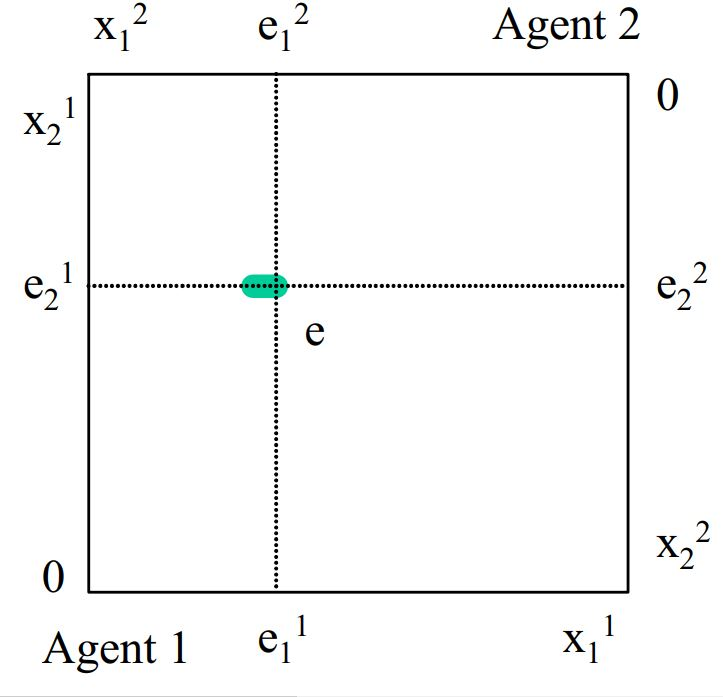
\includegraphics[scale=0.35]{images/edge01}
\end{center}

Now that we've established the both agents' consumption quadrant are represented in the box, we can go on and represent their preferences in the form of their utility functions. We'll use the typical indifference curves to do so and hence keep working with the concept of utility maximization, marginal rate of substitution, etc. \begin{center}
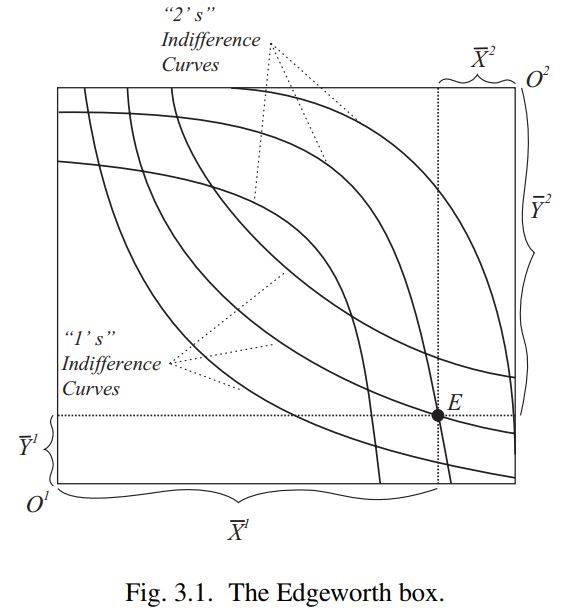
\includegraphics[scale=0.45]{images/edge02}
\end{center}

The endowment point $E$ is located on the intersection of two indifference curves. The area located inside the lens-shaped figure created by both indifference curves contains all points that are Pareto improvements of $E$. In the graph above, moving inside this area means that agent 1 is willing to give up an amount of good $X$ in exchange of more good $Y$. The opposite is true for agent 2. The fact that the area of the lens is non zero means that there is room for trade. Nevertheless, moving inside the lens does not mean that we have achieved a definitively better situation. Take for example a move to point $A$ in the graph below: there is still room for trade (i.e. the new lens is still not zero). The situation represented by point $B$ has no lens, hence it is Pareto-optimal! What is the difference between $A$, $E$ and $B$? The MRS of the two players are not equal in $A$ and $E$ whereas $B$ has this property of having equal MRS.

\begin{center}
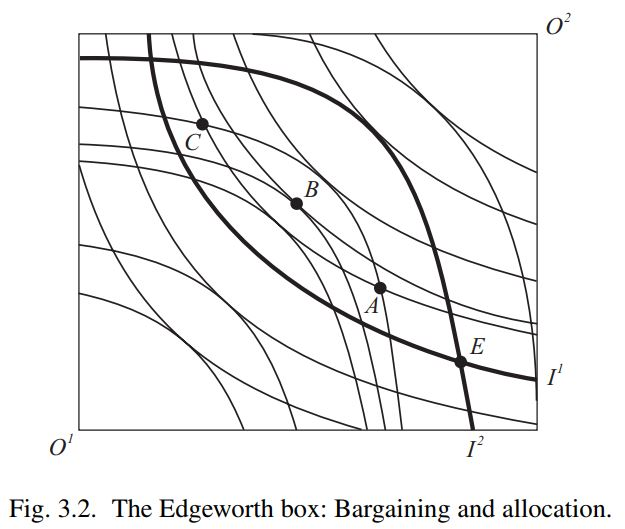
\includegraphics[scale=0.55]{images/edge03}
\end{center}

\subsection{Calculating an efficient allocation}

The tangency of indifference curve is what determines the optimality of a situation (in the Pareto sens). It is therefore important to characterize formally the set of all such allocations.

\begin{definition}[Pareto set]
All allocations within the Edgeworth box that satisfy: $$MRS_{x_1^1,x_2^1}^1 = MRS_{x_1^2,x_2^2}^2 $$ are allocations that are both feasible and Pareto optimal. We call this set of allocations the Pareto set.
\end{definition}

To compute the Pareto set, we'll solve the analytically equivalent problem of maximizing the utility of one agent for a given Pareto allocation for the other agent. We are looking for $$ x^{1*} \in \operatorname{arg}\max_x u^1(x) \text{ s.t. } \{u^2(x^2) = u^2(x^{2*})\} \text{ and } \left\lbrace\sum_{i=1}^{I} x_l^i \leq \sum_{i=1}^{I} e_l^i \quad \forall l =1,2\right\rbrace $$ First, notice that the two resource constraints can be plugged into the utility constraint since $x_l^2 = e_l - x_l^1$. Let's set up the Lagrangian: $$L\equiv u^1(x_1^1, x_2^1) + \lambda\left[u^2(e_1 - x_1^1, e_2 - x_2^1) - u^{2*}\right] $$ which has the following conditions: $$ \frac{\partial u^{1}}{\partial x_1^1} -\lambda \frac{\partial u^{2}}{\partial x_1^1} = 0 $$ $$\frac{\partial u^{1}}{\partial x_2^1} -\lambda \frac{\partial u^{2}}{\partial x_2^1} = 0 $$ which can be simplified to $MRS_{1,2}^1 = MRS_{1,2}^2$.

\begin{definition}[Contract curve]
The contract curve is the set of Pareto optimal allocations that can be achieved through voluntary negotiations starting from the endowment point. In other word, it is the set of Pareto optimal allocations that give higher utility than the endowment allocation. 
\end{definition}

\begin{center}
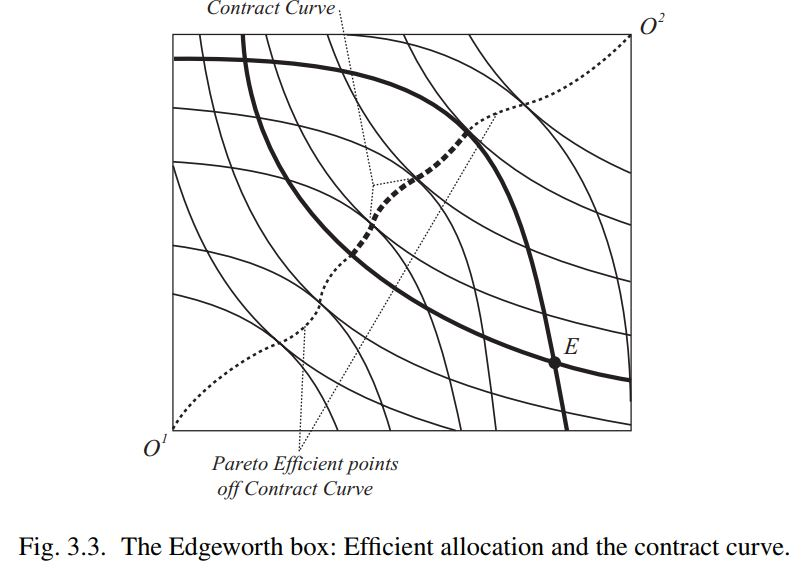
\includegraphics[scale=0.55]{images/edge04}
\end{center}

\subsection{Competitive market solution}

We have seen how to recover points that are Pareto optimal in the Edgeworth box. In order to find possible Walrasian equilibria, we still need to add the price system to the picture. In order to do that, we'll find all allocations chosen by each agent for all price vectors, such that markets clear out. Therefore, agent $i$'s problem is: $$x^{i*} \in \operatorname{arg}\max_x u^i(x) \text{ s.t. } p\cdot x^i = p\cdot e^i $$ Because we added the endowments in the budget constraint, the budget set will be defined as the area below the straight line of slope $-p_1/p_2$ passing through the endowment point $E$. Because of that constraint, we can rewrite our maximization problem as: $$x^{i*} \in \operatorname{arg}\max_x u^i(x_1, \frac{p\cdot e^i - p_1 x_1 }{p_2} )$$ This problem has the following condition: $$\frac{\partial u^i}{\partial x_1} - \frac{p_1}{p_2}\frac{\partial u^i}{\partial x_2} = 0 $$ which is equivalent to the following equation: $MRS_{1,2}^i = \frac{p_1}{p_2}$

\begin{definition}[Offer curve]
The offer curve of an agent is the set of optimal allocations, achievable from the endowment, for all price vectors. Hence, it satisfies: $$MRS_{1,2}^i = \frac{p_1}{p_2}$$ It represents what allocation an agent would choose for a given price vector.
\end{definition}

\begin{center}
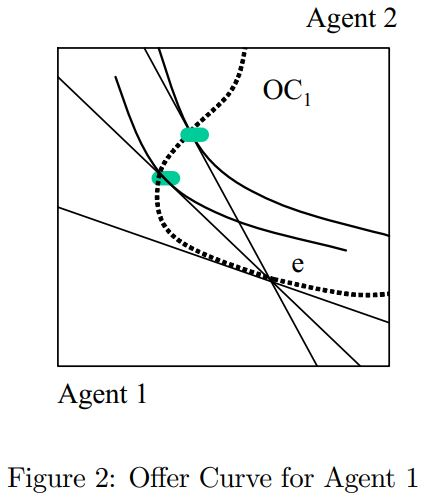
\includegraphics[scale=0.43]{images/edge05}
\end{center}

Finally, we can define the competitive (Walrasian) equilibrium in the Edgeworth box as the crossing between both offer curves. Indeed, if both offer curves cross at a given point, it must be that both $MRS$ are equal to the price ratio, as well as to each other! \begin{center}
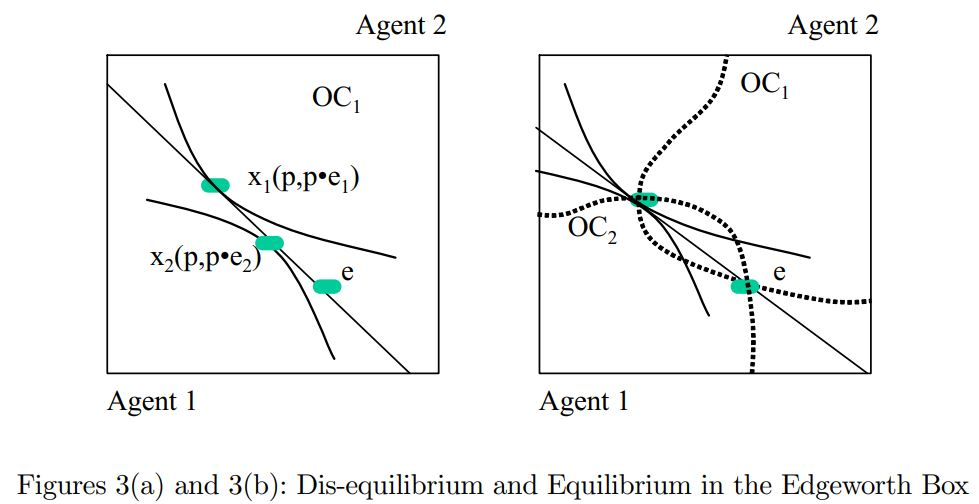
\includegraphics[scale=0.45]{images/edge06}
\end{center}

\section{Welfare theorems}

We have seen from the previous section that in the Edgeworth box, a competitive equilibrium must be on the Pareto set and hence must be Pareto optimal. In this section we will dig deeper into the relation between both concepts.

\begin{theorem}[First Welfare Theorem]
Let $(p, (x^i))$ be a Walrasian equilibrium for the economy $\mathcal{E}$. Then, if $u^i$ is increasing in $x$ for all $i$, the allocation $(x^i)$ is Pareto optimal.
\end{theorem}
\begin{proof}
Suppose there exists a feasible allocation $(\tilde x^i)$ such that $u^i(\tilde x^i) \geq u^i(x^i)$ for all $i$ and for some $i$: $u^i(\tilde x^i) > u^i(x^i)$. Then, since $u^i$ is increasing, it must be that $\tilde x^i \geq x^i$ for all $i$ and for some $i$: $\tilde x^i > x^i$. Because $(x^i)$ is a Walrasian equilibrium, we know that it exhausts the budget constraint completely, therefore it must be that for some $l$, we have $\sum_{i = 1}^{I} \tilde x_l^i > \sum_{i = 1}^{I} x_l^i = \sum_{i = 1}^{I} e_l^i $. And $(\tilde x^i)$ is not feasible: a contradiction.
\end{proof}

This result is quite interesting in the sense that it proves a very important phenomenon arising in decentralized economies: they are Pareto efficient. With pretty weak assumptions we have managed to show that a given number of agents acting only in their interests (Walrasian equilibrium) will achieve a desirable outcome (more like an outcome that no one can deviate from). Nevertheless, one should recall the underlying assumptions of the model which are not typically restated in the theorem, namely the price-taking assumptions, the existence of markets, prices are the same for everyone, etc. More importantly, nothing is said on how the agents achieve this equilibrium in a decentralized manner.

While the first welfare theorem gives us insight on how Walrasian equilibria are optimal, the second welfare theorem shows that under given prices and endowments, Pareto optimal outcomes are Walrasian equilibria.

\begin{theorem}[Second Welfare Theorem]
\end{theorem}


\chapter{Existence of GE}

Now that we have defined and looked at the consequences of the general equilibrium, we need to prove it exists. Indeed, if you look closely, the two welfare theorems assume the existence of equilibria in order to analyze their consequences, but do such equilibria exist? This is the question this chapter is trying to solve.

In particular, we've defined an equilibrium as a set of prices and quantities such that markets clear. In other terms, showing that an equilibrium exists is equivalent to finding a price vector such that $x_l(p_1, ...,p_L)$, the aggregate demand for good $l$ as a function of all prices is equal to the aggregate endowment in good $l$. And this for any $l\in 1, ..., L$. Arrow and Debreu proved in a one of the most important paper of economics, published in 1953. The theorem goes as follows.

\begin{theorem}[Existence of General equilibrium]
Given an economy $\mathcal{E}$, such that for all agents $i$:\begin{itemize}
\item $u^i(\cdot)$ is continuous.
\item $u^i(\cdot)$ is increasing.
\item $u^i(\cdot)$ is concave.
\item $e^i \gg 0$: everyone has at least a bit of everything in their endowment.
\end{itemize}
There exists a Walrasian equilibrium denoted by $(p^*, x^*)$.
\end{theorem}

The following sections will prove this result.

\section{Excess demand correspondences}

\begin{definition}[Excess demand correspondence]
For an agent $i\in 1, ..., I$, the excess demand correspondence $z^i:\mathbb{R}^L\twoheadrightarrow  \mathbb{R}^L$ is defined as: $$z^i(p) = x^i(p, pe^i) - e^i $$ where $x^i(p, pe^i)$ is the demand correspondence. The aggregate excess demand correspondence $z:\mathbb{R}^L\twoheadrightarrow  \mathbb{R}^L$ is: $$ z(p) = \sum_{i=1}^{I}z^i(p)$$
\end{definition}

Then the problem reduces to finding a $p^*$ such that $z(p^*) = 0$. The equilibrium characterized by $(p^*, x^i(p^*,p^*e^i)$ will then be a Walrasian equilibrium. Does such a point exist?

\chapter{Core of an economy}

Recall the structure of an exchange economy. Consumers are characterized by their endowments and preferences. We consider a finite set of consumers $I$, with a consumption determined by the positive quadrant $\mathbb{R}^L$. Each consumer $i\in I$ has endowment $\omega^i$ and preferences represented by utility function $u^i:\mathbb{R}^L\to\mathbb{R}$. An allocation $x^i\in\mathbb{R}^L$ is an assignment of $L$ goods to consumer $i$. We say that an allocation is feasible if $\sum_i x_l^i \leq \sum_i \omega_l^i $ for all $l\in L$. Finally, we assume that preferences satisfy LNS, continuity and strict convexity.

\section{Core of an exchange economy}

The main conceptual difference of the core with respect to the market equilibrium resides in the idea of bargaining. Each consumer owns their endowment and can use it for whatever purpose. Any feasible allocation (think of the Edgeworth box) can be proposed by/to the consumers. The concept of bargaining that will define the core in this economy is that groups of consumer can form coalitions, in which they can trade between themselves and achieve feasible allocations on their own, inside their own coalition. If a coalition can achieve a better allocation than the one proposed by/to the whole economy, they can withdraw from the proposed allocation and form their own economy. This threat is credible since all members in the coalition would actually prefer (or be indifferent) to leave the economy. An allocation that cannot be sustained is said to be blocked by a coalition of $S\subset I$ consumers; if there are no possible coalitions to block the allocation, it is said to be in the core. Now that the intuition has been explained, let's define all these terms in a more formal way.

\begin{definition}[Coalition]
A coalition is any subset $S\subseteq I$. Denote the size of $I$ by $n$ the number of consumers, there are $2^n - 1$ possible coalitions in an economy of $n$ consumers (note that the empty set cannot be part of a coalition).
\end{definition}

\begin{definition}[Blocking coalition]
An allocation $x = (x^1, x^2, ..., x^I)$ is said to be blocked by a coalition $S$ if there exists an allocation $x'$ such that $x^{'i} = x^i$ if $i\not\in S$ and for all $i\in S$:\begin{itemize}
\item $\sum_{i\in S} x_l^{'i} \leq \sum_{i\in S} \omega_l^{i}$ holds for all $l$, meaning that $x'$ is feasible inside (and outside) the coalition.
\item $x^{'i}\succeq x^i$, meaning that all consumers in the coalition weakly prefer the blocking allocation.
\item $x^{'j}\succ x^j$, for at least one $j\in S$, meaning that there exists at least one individual in the coalition who strictly prefers the blocking allocation.
\end{itemize}  
\end{definition}

In words, this definition formalizes the intuition that was described before: if a group of consumers can achieve a better allocation by themselves, they will not be interested in pursuing the allocation proposed by the economy. This makes the definition of the core pretty straightforward:

\begin{definition}[Core allocations]
The core of the economy is the set of all feasible allocations that are not blocked by any coalition $S\subseteq H$.
\end{definition}

The core of an economy is a generalization of the concept of the contract curve that we have seen in Edgeworth boxes. In fact,\begin{itemize}
\item Any allocation in the core must be individually rational, meaning that it must yield a higher or equal utility than the endowment point. The intuition for that claim is fairly easy since if the proposed allocation did not satisfy this requirement for at least one consumer, this consumer could form a coalition and leave the economy with his endowment.
\item Any allocation in the core must be Pareto efficient. This follows from the fact that if this was not the case, then the coalition of all consumers could redistribute the allocations such as to make everyone weakly better off. This implies that, starting from a core allocation, we cannot improve the situation of one or more consumers without hurting at least one consumer.
\end{itemize}

If this definition adds a new concept to our understanding of an exchange economy, it does not help us draw any meaningful conclusions yet: does the core even exist? How does it relate to the market? etc. The following sections will draw upon those questions.

\section{Competitive equilibrium and the core}

Recall the definition of a competitive equilibrium as being an allocation and a price vector such that, for all $i\in I$:\begin{itemize}
\item The allocation is individually affordable: $px^i\leq p\omega^i$.
\item The allocation is weakly preferred to any other allocation in the budget set: $x^i\succeq x^{'i}$ for all $x^{'i}$ in the budget set.
\item The allocation is feasible.
\end{itemize}

Now, under some assumptions, we set up the main theorem about core allocations: all competitive equilibria must be in the core.

\begin{theorem}
Let the economy satisfy the assumptions of unboundedness, local nonsatiation and strict convexity of preferences. Let $(p, x)$ be a competitive equilibrium, then $x$ is in the core of the economy.
\end{theorem}

\begin{proof}
By contradiction, suppose an equilibrium allocation is not in the core. Then there exists a blocking coalition $S\subseteq I$ and a blocking allocation $\tilde x$. From the definition of a competitive equilibrium under these particular preferences, it must be that, for all $i$, $ p x^i = p \omega^i $ and $x^i \succeq \hat x^i$ for all $\hat x^i$ such that $p \hat x^i \leq p \omega^i$. In parallel, from the definition of a blocking coalition we have that $ p \tilde x^i \leq p \omega^i \Leftrightarrow \sum_{i\in S} px \leq \sum_{i\in S} p\omega^i$ since all $\tilde x^i$ are in the budget set. For $\tilde x$ to be a blocking coalition, we need that for at least one individual $j$, $\tilde x^j\succ x^j$, which is not possible inside the budget set. Therefore, it cannot be true that there exists a blocking coalition to $x$: $x$ must be in the core.
\end{proof}

\section{Large economies and the core: replication}

This section deals with how the economy changes as the number of agents increase. To make the number of agents grow, we replicate the economy. Replication is allowing for each type of consumers that were exisiting before to be multiplied by a number $N$. If the economy had $I$ consumers, its $N$-replica has $N\times I$ consumers, with $N$ consumers of each type $i\in I$, with endowment $\omega^i$ and preferences $\succeq_i$. We will therefore denote each consumer in this economy by its type $i$ and number $n$: an allocation becomes $x = (x^{1,1}, x^{1,2}, ..., x^{1,n}, ..., x^{I,N})$.

\subsection{Equal Treatment property}

At first, it seems that multiplying the number of consumers is going to make the problem more and more difficult to analyze. However, as we'll see with the following theorem, the replication method makes it very easy to keep the economy fairly easy to work with. In fact, the theorem, called equal treatment property of the core implies that for all $i$ types in the economy, it must be that each of the $N$ individuals of each type is treated equally, that is for all $i$, $x^{i,q} = x^{i,q'}$ for any $q,q'\in N$.

\begin{theorem}
Assume consumer preferences follow local non-satiation, strict convexity and continuity. Let $x$ be in the core of the $N$-replica of the economy, then for all $i$, $x^{i,q} = x^{i,q'}$ for any $q,q'\in N$.
\end{theorem}

\begin{proof}
Recall that the core allocation must be feasible: $\sum_{i\in I}\sum_{q\in N} x^{i,q} \leq \sum_{i\in I}\sum_{q\in N} \omega^{i}$ or equivalently, $ \sum_{i\in I}\frac{1}{N}\sum_{q\in N} x^{i,q} \leq \sum_{i\in I} \omega^{i}$. Now, by contradiction, suppose the theorem does not hold, that is, that for some $i$, we have $q,q'$ such that $x^{i,q} \neq x^{i,q'}$. For each type, we'll denote as $x^{i^*}$ the least preferred allocation in the core: the allocation that yields the lowest utility in each type. Note that for the types $j$ that have equal treatment: $x^{j^*} = x^{j,q}$. Without loss of generality, let's rank the consumers in each types so that $q=1$ implies that the consumer has indeed the worst allocation of his type.

In each type, the average allocation $\bar x^i = \frac{1}{N} \sum_{q\in N} x^{i,q} $ has to be weakly preferred by the individual $q=1$. Consider the coalition $S$ of all individuals $q=1$, from the feasability constraint above, it must be that: $$ \sum_{i\in S}\frac{1}{N}\sum_{q\in N} x^{i,q} \leq \sum_{i\in S} \omega^{i} $$ $$\sum_{i\in S} \bar x^{i} \leq \sum_{i\in S} \omega^{i} $$ which implies that the average allocation discussed just above is achievable inside the coalition of all worse off consumers off each types: a contradiction.
\end{proof}

\subsection{Core convergence}



\chapter{GE in production economies}

\section{Firms and production technoloogy}

We'll define a firm as an entity with a name $j\in 1,2,..., J$, a production technology represented by its production set $Y_j \subset \mathbb{R}^L$, and the people who own a share $\theta_{ij}$ of it such that $\sum_{i=1}^{I} \theta_{ij} = 1 $. The set $Y_j$ representing the production set is a $L$-dimensional vector containing inputs (negative values) and outputs (positive values). The more common way to represent the production set is via its production function $y = f(x)$ where $x$ are the inputs and $y$ is the output. As such, the function represents the boundary of the production set as $y \leq f(x)$. Graphically, a production set looks like the following figure:\begin{center}
 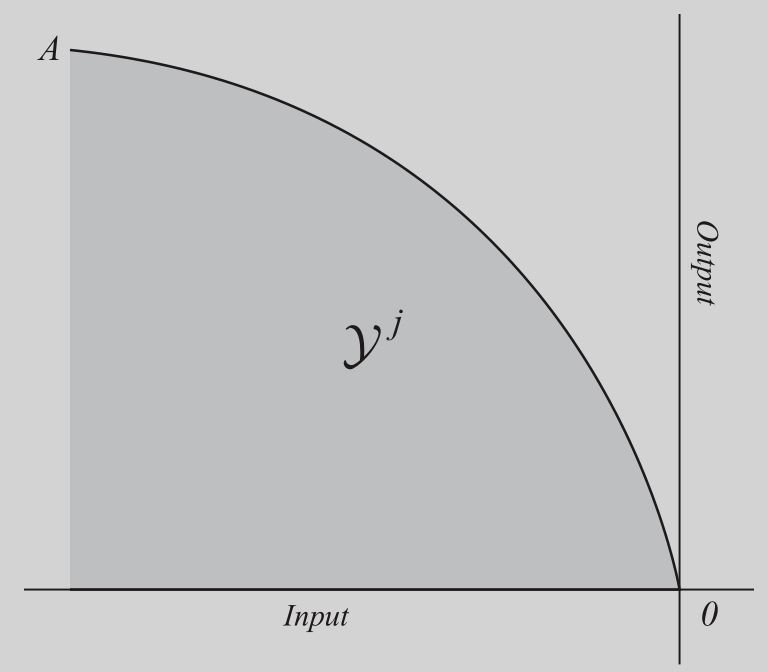
\includegraphics[scale=0.25]{IMAGES/prodset.JPG}
 \end{center} 

For better properties of our model, we'll assume that, for all $j$, $Y_j$ is nonempty, convex and closed, and that the zero vector is included in $Y_j$. We further assume that there is free disposal (i.e. all $y < f(x)$ are in $Y_j$. Note that assuming a convex production set is implying that returns to scale will be either constant or decreasing. In the particular case of constant returns to scale and competitive firms, profits will be 0, hence $\theta_{ij}$ won't matter in our analysis.

A supply correspondence for a firm will be the set of vector of quantities of goods it's willing to buy and supply for a given price vector. We continue to describe prices as a vector $p\in\mathbb{R}^N$. Furthermore, we'll assume that all firms are price-takers, meaning that the price vector is exogenous to their maximization problem. Then, the supply function is really the solution of the firm's profit maximization problem and we can write: $$ S_j(p) = \{ y_j^* : y_j^*\in Y_j, p\cdot y_j^*\geq p\cdot y \ \ \forall y\in Y_j\} $$ or in words, the supply correspondence is the set of all combinations of goods inside the production that yield the maximum amount of profits. Analogous to the consumer side, we define aggregate supply as the sum of all firms' supply correspondence: $S(p) = \sum_{j=1}^{J} S_j(p) $. 

\section{Market Equilibrium}

Now that we have seen how the new agents of the model behave, we can bring back our consumers from the previous chapters to close our model.

\begin{definition}[Feasible allocation in a production economy]
We define a feasible allocation for a production economy as a list of the goods demanded $x = (x_1, ..., x_I)$ and goods supplied $y = (y_1, ..., y_J)$ such that:\begin{itemize}
\item[i.] For all $i$, $x_i \in X_i$
\item[ii.] For all $j$, $y_j \in Y_j$
\item[iii.] For all $l$, $\sum_{i=1}^{I} x_{il} = \sum_{i=1}^{I} \omega_{il} + \sum_{j=1}^{J} y_{jl} $
\end{itemize}
\end{definition} 

We have seen in the exchange economy how for given price vectors, a feasible allocation may or may not be a market equilibrium where the equilibrium notion was defined for consumers only. Here we extend this definition to the firms:\begin{definition}[Market equilibrium for a production economy]
In a production economy, a market equilibrium is a list $(p, x, y)$ where $p$ is a normalized price vector such that $p\in\Delta^L$ and $(x,y)$ is a feasible allocation such that:\begin{itemize}
\item[i.] For all $i$, $x_i$ is affordable, $p x_i \leq p \omega_i + \sum_{j=1}^{J} \theta_{ij}\cdot p y_j $ and yields the highest utility among all affordable goods at price $p$.
\item[ii.] For all $j$, $y_j$ is achievable, $y_j\in Y_j$ and yields the highest profit among all achievable production plans.
\end{itemize}
\end{definition}

We can also replicate the first and second welfare theorems in the general equilibrium with production.

\begin{theorem}[First Welfare Theorem in a production economy]
Suppose that for all $i\in I$, $u_i(\cdot)$  satisfies LNS. Then, if a combination of a price vector $p$ and an allocation $(x,y)$ constitute a market equilibrium, the allocation $(x,y)$ is Pareto-efficient.
\end{theorem}

\begin{proof}

\end{proof}

\begin{theorem}[Second Welfare Theorem in a production economy]
Let $(x,y)$ be a Pareto-efficient allocation. Suppose that $X_i$ is non-empty and convex, $u_i$ is continuous, quasi-concave and satisfies LNS. Moreover, $x_i\in \operatorname{int}(X_i)$. Suppose that $Y_j\subset \mathbb{R}^L$ is nonempty, closed and convex, satisfies free-disposal and inaction. Then, there exists a price vector $p$ such that $(p, x,y, W)$ is a market equilibirum with transfers. 
\end{theorem}

\chapter{Uncertainty in complete/incomplete markets}

As in the previous chapters, this last chapter will use an economy with $I$ consumers, $L$ goods and $J$ firms. However, we also add uncertainty to the model, introducing different states of the world (or realizations of the economy).

\section{Economy with uncertainty}

A state of the world is to be understood as a description of one possible outcome of the economy. We assume that there is an exhaustive set of states of the world $S$ (containing $S$ elements). We'll use this set to (re)define our economy in a state-contingent way.

\begin{definition}[State-contingent commodities]
For every commodity $l\in L$ and state of the world $s\in S$, the allocation $x_{ls}$ represents the allocation of good $l$ that is to be received if the particular state of the world $s$ turns out to be realized. This yields the following (long) notation for the description of the whole economy under uncertainty: $$ x = (x_{11}, x_{12}, ..., x_{ls}, ..., x_{LS}) $$
\end{definition}

\begin{definition}[State-contingent endowments]
In the same way as with commodities, endowments are defined for any $i$ as an allocation of $L$ goods in all $S$ states of the world so that: $$\omega_{i} = (\omega_{11i}, ..., \omega_{LSi}) $$ meaning that if the state of the world $s$ occurs, consumer $i$ receives the endowment $\omega_{is} = (\omega_{1si}, ..., \omega_{Lsi})$. If $\sum_{i\in I}\omega_{is} = \sum_{i\in I} \omega_{is'}$ for all states of the world $s,s'\in S$, we say that there is no aggregate uncertainty: the amount of resources available in the economy is not state-contingent.
\end{definition}

\begin{definition}[State-contingent production plan]
We can define a production plan dependent on states of the world in the same way as the two previous objects. We define the technological possibilities of the firm $j$ as a production set $Y_j\subset \mathbb{R}^{L\times S}$. Hence, the vector $y_j \in Y_j$ if for any state of the world $s$: $$y_{sj} = (y_{1sj},..., y_{Lsj}) \in Y_{sj} $$
\end{definition}

Finally, we will define how preferences of consumers change under uncertainty. This chapter does not cover a complete discussion on the topic since it will be done more in depth in class 7741, but we use a simple, straightforward functional form that applies nicely to our new conceptual economy: the expected utility.

\begin{definition}[Expected (or Bernouilli or vNM) utility function]
Let all consumers in the economy hold beliefs about the probability with which each state $s$ can occur, and denote this belief $\pi_{si}$ as the probability (subjective to $i$) that the state $s$ will occur. We already know how the utility function in each state looks like $u_{si}(x_{1si}, ..., x_{Lsi})$ is no different that the utility functions we have used before.
Then the utility of a complete $x$ allocation is given by: $$u_{i}(x_i) = \sum_{s\in S} \pi_{si}u_{si}(x_{1si}, ..., x_{Lsi}) $$ $$\text{and } x_i\succeq \tilde x_i \Leftrightarrow u_{i}(x_i)\geq u_{i}(\tilde x_i) $$
\end{definition}

\section{Arrow-Debreu equilibrium}

Describing a general equilibrium in such conditions is expectedly harder than without uncertainty, that's why we will make a strong assumption form the beginning, to ensure that we can parallel the equilibrium with uncertainty to the previous general equilibrium concepts discussed: we assume that at time $t=0$, when consumers exchange, firms produce, etc., before the uncertainty has cleared, there exists as market for all goods in all states of the world. This means that you can buy a commodity $l$ in state $s$ at a price denoted $p_{ls}$ before even knowing for sure that $s$ will realize. Observe that in this case, the payment you make is not state-contingent (you pay whether you observe $s$ or not), but the delivery of the good is (you receive $x_{ls}$ only if $s$ occurs). This (strong) assumption implies that this model is in fact a generalization of the economy we've studied before, with one additional dimension. And in fact, we'll show that the notion of competitive equilibrium in an economy without uncertainty is simply a particular case of the more general equilibrium studied here: the Arrow-Debreu equilibrium.

\begin{definition}[Arrow-Debreu equilibrium]
An allocation $(x_1^*, x_2^*, ..., x_I^*, y_1^*, y_2^*, ..., y_J^*)\in \mathbb{R}^{LS(I+J)}$ and a system of prices for contingent goods $p^* = (p_{11}, ..., p_{LS})\in \mathbb{R}^{LS}$ is an Arrow-Debreu equilibrium if:\begin{itemize}
\item For all $j\in J$, $p^*y_j^*\geq p^*y_j$ for any $y_j\in Y_j$: $y_j^*$ is the production plan consisting of the profit maximizing allocation in each state $s$, at the given price vector.
\item For all $i\in I$, $x_i^*\succeq x_i$ for any $x_i$ in the budget set: $x_i^*$ is the allocation consisting of the most preferred allocations in each state, at the given price vector.
\item $\sum_{i\in I} x_i^* = \sum_{j\in J} y_j^* + \sum_{i\in I} \omega_i $: the equilibrium allocation is feasible in all states of the world.
\end{itemize}
\end{definition}

In order to understand this new concept of equilibrium, let's focus on a quite simple example of a small exchange economy of $I = 2$ consumers, $L = 1$ commodity and $S=2$ states. Observe that here $S\times L = 2$ so we can represent this economy in an Edgeworth box where we display the good in state $2$ vertically, while the good in state $1$ will be on the horizontal axis. Further assume that if state $1$ occurs, consumer $1$ gets the unique unit of the good, while if state $2$ occurs, consumer $2$ will get the good. Since $\sum_i \omega_{1i} = \sum_i \omega_{2i}$, there is no aggregate uncertainty. Now, the most important part to finding an Arrow-Debreu equilibrium in this economy is to define the utility functions. We know that they follow a vNM functional form so that: $u_i = \pi_{1i}u_{1i}(x_{1i}) + \pi_{2i}u_{2i}(x_{2i})$. As we did before, we can characterize the Pareto set as the set of points where both MRS are equal, here: $$\frac{\partial u_1/\partial x_{11}}{\partial u_1/\partial x_{21}} = \frac{\partial u_2/\partial x_{12}}{\partial u_2/\partial x_{22}}$$ 
$$\frac{\pi_{11}u_{11}'}{\pi_{21}u_{21}'} = \frac{\pi_{12}u_{12}'}{\pi_{22}u_{22}'}$$ This equation can get pretty messy with 4 different utility functions but an usual assumption is that the utility function form is not state-contingent: $u_{1i}(\cdot) = u_{2i}(\cdot)$, and hence, if $x_{1i} = x_{2i}$, we have that $u_{11}' = u_{21}'$. Moreover, note that if $x_{1i} = x_{2i}$, then $x_{1j} = x_{2j}$ in the two consumers case. Hence on the 45-degree line of the box, the MRS of consumer $i$ is: $\pi_{1i}/\pi_{2i} = \frac{\pi_{1i}}{(1 - \pi_{1i})}$. This result implies that we can find the Pareto set by comparing subjective probabilities of both consumers:\begin{itemize}
\item If both consumers expect state $1$ to occur with the same probability, $\pi_{11} = \pi_{12}$, then the 45-degree line has both MRS equal: the 45-degree line is the Pareto set.
\item If consumer $1$ expects one state to occur with a higher probability than consumer $2$, $\pi_{11} > \pi_{12}$, then the 45-degree line has the MRS of consumer $1$ higher than the one of consumer $2$: consumer $1$ values good $1$ more than consumer $2$, we move to the bottom-right and the 45-degree line must be above the Pareto set.
\item If consumer $2$ expects one state to occur with a higher probability than consumer $2$, $\pi_{11} < \pi_{12}$, then the 45-degree line has the MRS of consumer $1$ lower than the one of consumer $2$: consumer $2$ values good $1$ more than consumer $1$, we move to the top-left and the 45-degree line must be below the Pareto set.
\end{itemize}

The last equilibrium was fairly easy to characterize as  we had no aggregate uncertainty (square Edgeworth box) and state-independent utilities. For the following example, let's assume that there is aggregate uncertainty but keep with the same utility functions. In particular, we assume that the total endowment in state 1 is equal to 2 units of the good, while in state 2 we still have only one unit. This time there are two 45-degree line to observe: for consumer 1, if $x_{11} = x_{21}$, we have that $x_{12} = 2 - x_{11} > x_{22}$, hence, $\operatorname{MRS}^1 > \operatorname{MRS}^2$ for the same beliefs and the Pareto set must be to the bottom-right; for consumer 2, the same reasoning shows that the Pareto set must at the top-left of his 45-degree line. Therefore, for the same beliefs, the Pareto set must be lying between both 45-degree lines. This result implies that for both consumers, at the equilibrium, $x_{1i}>x_{2i} \Leftrightarrow u'_{1i} < u'_{2i}$ meaning that the $\operatorname{MRS}^i < \frac{\pi_{1i}}{\pi_{2i}}$. And finally, because in a competitive equilibrium $\operatorname{MRS}^i = \frac{p_1}{p_2}$, we have that in an Arrow-Debreu equilibrium, it is always the case that: $$\frac{p_1}{p_2} < \frac{\pi_{1i}}{\pi_{2i}} $$

\section{Sequential Trade, Asset Markets and the Radner equilibrium}



\end{document}